\chapter{Votre premier diagramme}
\section{Introduction}
Ce chapitre va vous permettre de réaliser une vote premier diagramme avec LoCD en moins de 5 minutes  \smiley ! Voici le résultat que vous obtiendrez au terme : 
\begin{figure}[htbp]
  \centering
  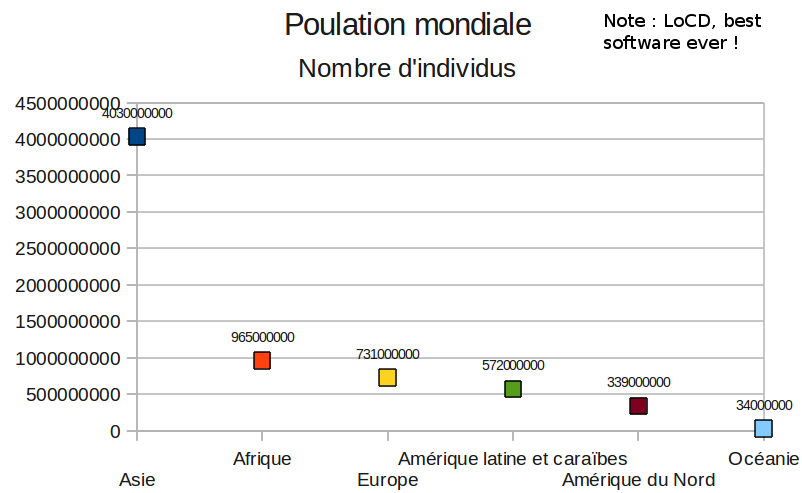
\includegraphics[scale=0.60]{img/diagrammenuages}
  \caption{Nuages de points avec toutes les méta données possibles renseignées}
  \label{fig:dnuages}
\end{figure}

\section{1\up{ère} \'Etape : Génération du fichier d'entrée}
Ouvrez un éditeur de texte de votre choix. Saisissez les lignes suivantes (utilisez le copier/coller pour gagner du temps).
\begin{verbatim}
  >TITLE: Les plus grands pays du monde pays (~2010)
  >SUBTITLE: En km²
  >Note: La France n'est que 42ème

  Russie      Canada 	   États-Unis    Chine 	    Brésil 
  17 098 242  9 984 670  9 629 091  	9 596 961   8 514 877 km2 	
\end{verbatim}
Enregistrez le fichier : \verb+mon_premier_diagramme.txt+
\section{2\up{ème} \'Etape : Utilisation de LoCD}
Il ne vous reste plus qu'a lancer la commande suivante :
  \begin{figure}[htbp]
    \centering
    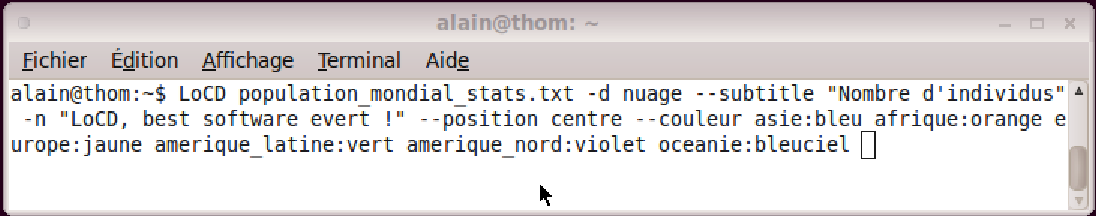
\includegraphics[scale=0.40]{img/ecommandes}
    \caption{Exemple d'utilisation de LoCD en ligne de commandes.}
    \label{fig:ecommandes}
  \end{figure} 
  
Et voilà avez crée votre premier diagramme avec LoCD ! Si vous avez rencontrez des difficultés au cours de ce chapitre, vous pouvez vous référer aux différentes parties de ne manuel qui détaille chaque étapes en détail.
